\section{A common use-case}
\subsection{Retry my results}

\begin{frame}{A classic use case}
\centering{
\onslide<1->{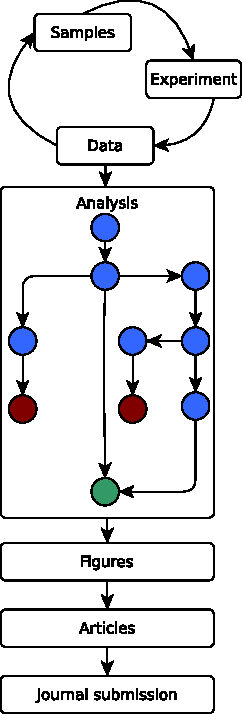
\includegraphics[width=0.17\textwidth]{images/schema_soumission_fair.pdf}}
\onslide<2->{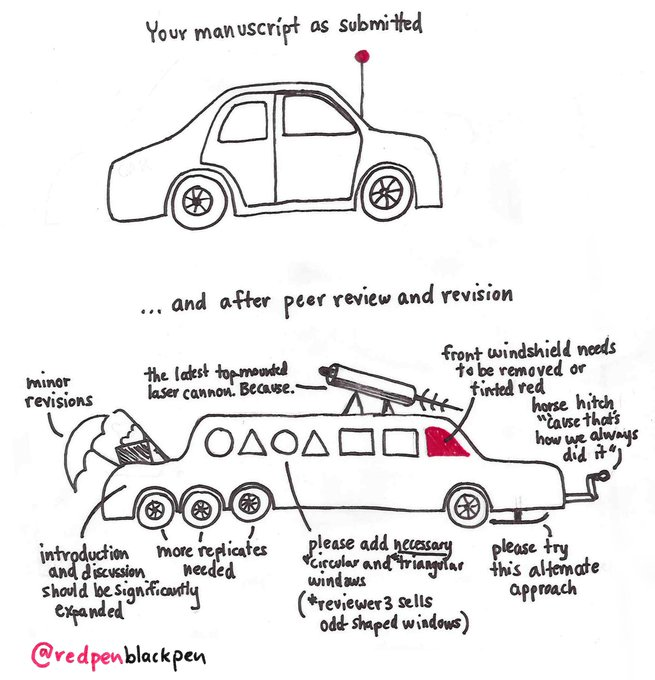
\includegraphics[width=0.4\textwidth]{images/review.jpg}}
\onslide<3->{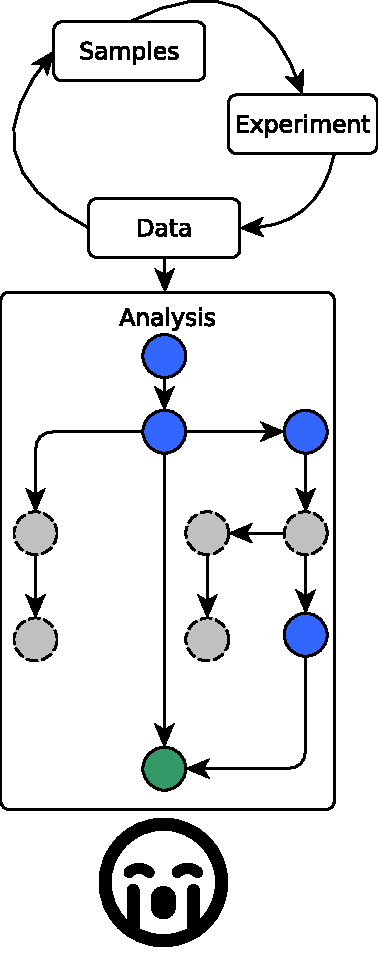
\includegraphics[width=0.17\textwidth]{images/schema_soumission_fair_echec.pdf}}}
\end{frame}
\begin{frame}{A classic use case}
\centering{What are the changes ?}
\begin{columns}
\column{.5\textwidth}
\begin{itemize}
	\item Tool version
	\item Packages
	\item Environment variables
\end{itemize}
\column{.5\textwidth}
\begin{itemize}
	\item OS version
	\item The computer 
	\item ...
\end{itemize}
\end{columns}
\end{frame}

\begin{frame}
\begin{itemize}
\item Tool compatibility troubles
	\begin{itemize}
	\item Python version ? 2.7, 3.8...
	\item Which tool version ?
	\item Installation without root access
	\item coexistance bewteen severals versions, libraries
	\end{itemize}
\end{itemize}
\end{frame}

\subsection{The use of packaging}
\begin{frame}[<+->]{Encapsulation levels}
\textit{Encapsulation: capture the environment of applications (OS, packages, libraries) to control their execution}
\begin{itemize}[<+->]
	\item Hardware virtualisation (virtual machines) 
\includegraphics[width=0.09\textwidth]{images/VM_logo.png} 
	\item OS virtualisation (images and containers) 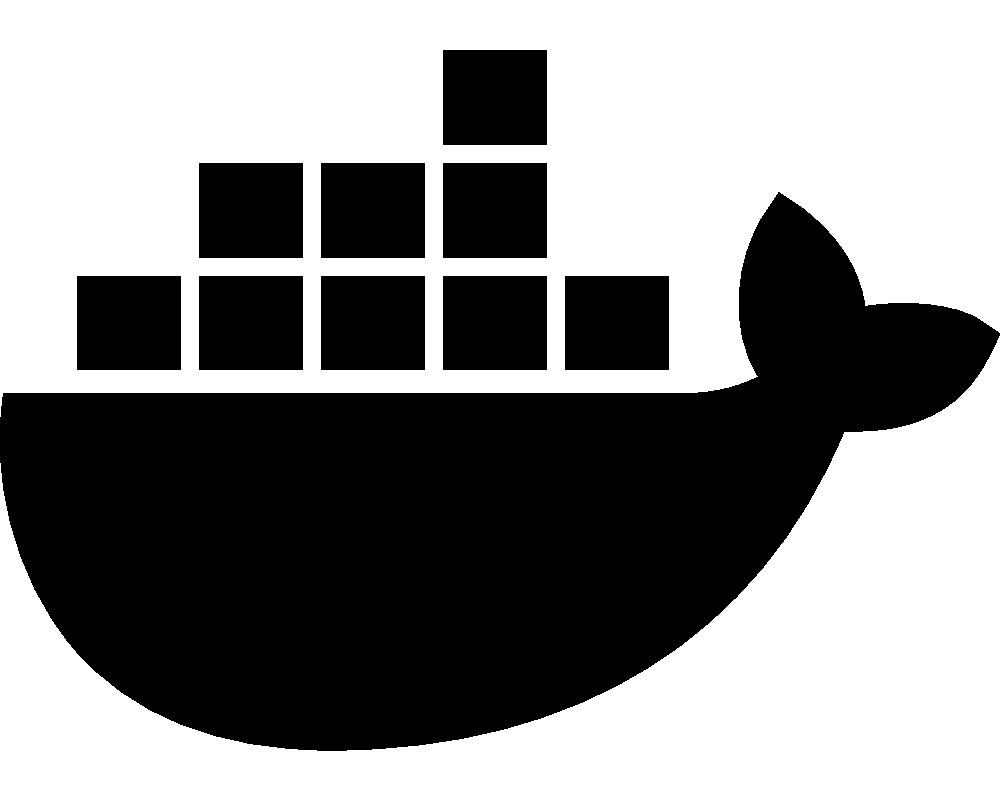
\includegraphics[width=0.09\textwidth]{images/docker.pdf} 
\includegraphics[width=0.09\textwidth]{images/singularity_logo.pdf} 
	\item Environment management (package manager) 
\includegraphics[width=0.09\textwidth]{images/conda_logo.pdf} 
\end{itemize}
\end{frame}

\subsection{Example with R}
\begin{frame}{Example of R and package installation}{Classical installation}
\begin{itemize}[<+->]
	\item Start with a computer and a specific OS
	\item Inside, we installed a new 
\includegraphics[width=0.3cm, height=0.3cm]{images/r-project.pdf} application
	\item 
\includegraphics[width=0.3cm, height=0.3cm]{images/r-project.pdf} need some dependencies
	\item we tested the last  
\includegraphics[width=0.3cm, height=0.3cm]{images/r-project.pdf} version --> might be conflicts
\end{itemize}

\onslide<1->{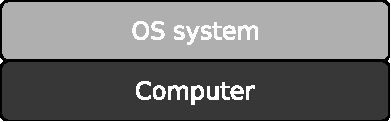
\includegraphics[width=0.25\textwidth]{images/conda_env_1.pdf}}
\onslide<2->{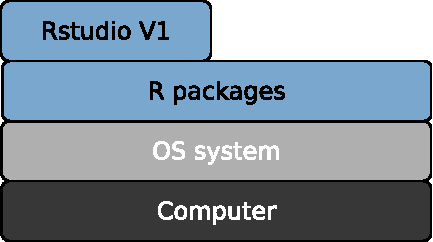
\includegraphics[width=0.25\textwidth]{images/conda_env_2.pdf}}
\onslide<3->{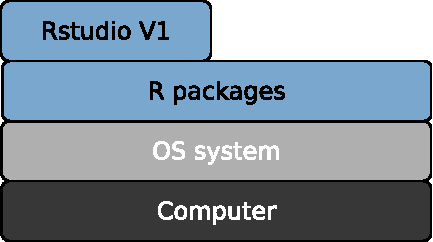
\includegraphics[width=0.25\textwidth]{images/conda_env_2.pdf}}
\onslide<4->{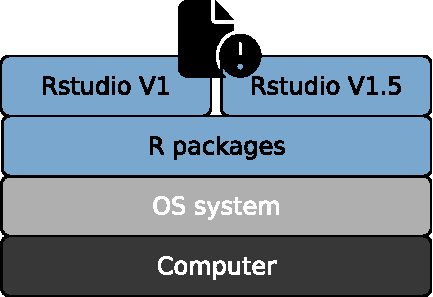
\includegraphics[width=0.25\textwidth]{images/conda_env_4.pdf}}
\end{frame}

%% A METTRE EN FIN DE DIAPO
\begin{frame}[<+->]
Some recommandations \footnote{Recommendations for the packaging and containerizing of bioinformatics software Gruening, F1000 Research, 2019. DOI 10.12688/f1000research.15140.2}
\begin{itemize}
\item A package first
\item One tool, one container
\item Tool and container versions should be explicit
\item Avoid using ENTRYPOINT
\item Reduce the size of your container as much as possible
\item Keep data outside of the container
\item Add functional testing logic
\item Check the license of the software
\item Make your package or container discoverable
\item Provide reproducible and documented builds
\item Provide helpful usage message
\end{itemize}
\end{frame}